% 这是有限群附录

\chapter{Finit Group}
这篇附录是根据李新征老师群论讲义个教学录像整理而成的笔记, 大致只打算写完有限群, 对于高量学习绰绰有余。
\section{群的基本结构}
\subsection{群的定义和一些基本定理}
其实在接受前面对于线性空间的抽象定义之后也很好接受群的概念:
\begin{define}{群的定义}
    群是一个有着\textbf{乘法}$\circ$这一特殊结构的元素集合$G$:
    \begin{itemize}
    \item[$\bullet$] \textbf{封闭性}:$\forall g_1,g_2\in G\rightarrow g_1\circ g_2\in G$
    \item[$\bullet$] \textbf{结合律}:$(g_1\circ g_2)\circ g_3=g_1\circ (g_2\circ g_3)$
    \item[$\bullet$] \textbf{单位元(幺元)存在性}:$\exists e\in G,\mathrm{s.t.}\forall g\in G\rightarrow g\circ e=e\circ g=g$
    \item[$\bullet$] \textbf{逆元存在性}:$\forall g\in G,\exists g^{-1}\in G\rightarrow g\circ g^{-1}=g^{-1}\circ g=e$
    \end{itemize}
\end{define}
上面的定义中不必额外强调单位元和逆元的唯一性, 因为根据定义唯一性自动存在。而且有\footnote{后面在不引起歧义时, 省略乘法符号}:
\begin{equation*}
    (g_1g_2)^{-1}=g_2^{-1}g_1^{-1}
\end{equation*}

不过要注意, 一般的群的乘法是\textbf{不满足}交换律的, \textbf{乘法额外满足交换律的群我们称之为Abel群}。
\begin{example}{群的例子}
    全体整数$\mathbb{Z}$在自然加法作为乘法的情况下构成一个群, 而且还是一个Abel群。
\end{example}
\begin{define}{群的阶}
    群的阶的定义和集合的势的概念是相通的, 定义为群内元素的个数, 记为$|G|$, 常说的有限群指的就是群的阶有限大。
\end{define}
下面要介绍的定理是后面的证明几乎都需要用到的定理:
\begin{theorem}{重排定理}
    \begin{equation*}
        gG=Gg=G
    \end{equation*}
    其中$g\in G$, 其实就是说$G$中拿出一个元素再去和$G$中的所有元素相乘, 得到的集合还是原来的群$G$本身, 而且不会出现重复。$g$的作用只是把原先的群元素重新排列了一下。
\end{theorem}
\begin{proof}
     $(1)\forall g_\alpha \in G$,由逆元存在性和封闭性知$g^{-1}g_\alpha \in G$,那么再根据结合律和逆元定义知$g(g^{-1}g_\alpha)=g_\alpha$,那么当
    $g_\alpha$取遍$G$中元素我们便得到了$gG=G$.\\
    $(2)$用到群相关定理证明的大杀器:{\color{red}{反证法}},设$g_\alpha\neq g_\beta$,如果$gg_\alpha=gg_\beta$,那么$g^{-1}(gg_\alpha)=g^{-1}(gg_\beta)\Rightarrow g_\alpha= g_\beta$,
    与已知矛盾.这一证明其实用掉了群的所有性质.\qed
\end{proof}
\subsection{群的内部结构}
\begin{define}{子群}
    设$H$是群$G$的一个子集, 如果$H$中的元素在$G$的乘法定义下也构成一个群, 那么就称$H$是$G$的一个子群, 记为$H\leq G$
\end{define}
\begin{example}{平庸子群}
    显然任何群$G$的幺元和其本身是$G$的两个子群,我们称之为平庸子群,其它的我们称为$G$的固有子群。
\end{example}
\begin{define}{循环子群和群元的阶}
    对任意一个\textbf{有限群}$G$,从中任取一个元素$a$,在原先的群乘法定义下作幂操作,\uwave{总是}可以得到一个$G$的子群$Z_k\equiv{a,a^2,a^3,\ldots,a^k=e}$,我们称之为
    $G$的一个循环子群,这个子群的阶,或者说使得$a^k=e$的最小的$k$称之为群元$a$的阶.
\end{define}
这里需要额外说明的就是为啥任何一个元素一定可以生成一个循环子群。只需要说明使$a^k=e$的$k$一定存在,$a=e$,问题解决;$a\neq e$,那么$a^2\neq a$否则$a=e$,$a^2=e$那么问题解决,
但如果$a^2\neq e$,就再考虑$a^3$,如此下去,由于前提是$G$为有限群,所以这个$k$一定存在。
\begin{define}{陪集}
    设$H\leq G$,由固定的$g\in G$可以生成$H$的左陪集:$gH\equiv{gh|h\in H}$,或是右陪集:$Hg\equiv{hg|h\in H}$
\end{define}
注意上面的定义中我们并没有用“群”这个字眼,说明陪集这个玩意一般只是一个集合而已,没有群结构。不难证明陪集中的元素是和子集$H$中的元素一一对应的,根据重排定理,
$g\in H$时$gH$和$Hg$构成一个群,就是$H$本身。
\begin{theorem}{陪集定理}
    $H\leq G, g_1,g_2\in G\rightarrow \{g_1H=g_2H\}\oplus \{g_1H \cap g_2H=\varnothing\}$\footnote[0]{其中$\oplus$表示“异或”,表示两者只能取其一。}
\end{theorem}
这个定理使用重排定理和反证法很好证明,只需要说明只要两个左陪集有一个公共元素那么$g_1H=g_2H$即可。当然,这个定理对于右陪集一样适用。这个定理也告诉我们或许任意一个群可以分解为一系列其某个子群的陪集的不交并。
\begin{proposition}{陪集分解}
    $H\leq G$,则$G$一定可以分解为一系列陪集的不交并,及:
    \begin{equation*}
        G=eH+g_1H+g_2H+\cdots
    \end{equation*}
\end{proposition}
根据前面的陪集定理,我们只需要在构建这个分解时,不断选取$g_\alpha$不属于前面的集合去构建新的陪集$g_\alpha H$即可。前面我们说过陪集元素和$H$一一对应,那么$|gH|=|H|$,再看陪集分解,由
于我们可以将任意一个集合分解为一系列陪集的\textbf{不交并},所以我们立即得到下面的Lagange定理:
\begin{theorem}{Lagrange定理}
    有限子群的阶必为群的阶的因子,也就是说$|H|$一定可以整除$|G|$
\end{theorem}
\begin{define}{共轭}
    $\forall f,h\in G$,如果$\exists g\in G$,使得$gfg^{-1}=h$,我们就称这两个元素共轭,记为$f\sim h$
\end{define}
群元素共轭的概念抽象一点这就是集合中的\textbf{等价关系的概念},满足下面三条:
\begin{itemize}
    \item[$\bullet$] \textbf{对称性}:$f\sim h\rightarrow h\sim f$
    \item[$\bullet$] \textbf{传递性}:$f_1\sim h,h\sim f_2\rightarrow f_1\sim f_2$
    \item[$\bullet$] \textbf{反身性}:$f\sim f$
\end{itemize}
上面的三条性质共轭全部满足,说的具体一点所有的$n\times n$矩阵构成一个群(这其实是个无限群),共轭的概念就是矩阵之间的相似概念。
\begin{define}{类}
    群$G$可按共轭关系分割成一些等价类$A_a={gag^{-1}|\forall g\in G}$.称$A_a$为群$G$的元素$a$的共轭类,简称为群的$a$类.
\end{define}
共轭类有下面的性质:
\begin{itemize}
    \item (1)单位元素$e$自称一类;
    \item (2)Abel群中的所有元素都自成一类;
    \item (3)类中的所有元素的阶都相等。
\end{itemize}

由于两个共轭类之间也有类似陪集之间的不相交的性质,所以我们也很容易实现将一个群用其群元的类来分解,只要对每个元素确定其类即可。不过前面的陪集分解是分解为一系列
大小相等的等份,而按照类的分解就不一定是等分了,不过还是有下面类似的定理:
\begin{theorem}{类中的元素个数}
    有限群的每个元素确定的类中的元素的个数都是群的阶的因子
\end{theorem}
\begin{proof}
    我们的目的是找到群的任意元素$g$确定的类的元素个数。

    证明这个定理的第一步是证明$\forall g\in G$,定义$H_g\equiv\{h\in G|gh=hg\}$,也就是所有与$G$中元素互易的元素构成了$G$的一个子群。由于子群乘法的定义来源于$G$,是良好定义的,
    所以我们只需要证明封闭性和逆元存在性。

    先证封闭:$gh_1=h_1g,gh_2=h_2g\rightarrow gh_1h_2=h_1gh_2=h_1h_2g$

    再证有逆:$gh=hg\rightarrow h^{-1}g^{-1}=g^{-1}h^{-1}\rightarrow gh^{-1}=h^{-1}g\rightarrow h^{-1}\in H_g$

    第二步是将$G$陪集分解为$\{g_0H_g,g_1H_g,\ldots\}$,其中$g_0$是幺元。注意到每个陪集$g_iH_g$中,$h_\alpha$取遍$H_g$,也就是$g_i h_\alpha$取遍$g_iH_g$中的所有元素时,
    $(g_i h_\alpha )g(g_i h_\alpha )^{-1}$给出的是和$g$共轭的元素这是毋庸置疑的,我们要是能进一步证明其实给出的还是同一个元素,我们记为$\tilde{g_i}$,我们就把陪集$g_iH_g$和$g$类中的元素
    对应起来了,如果不同的陪集给出不同的元素,也就说还可证明这种对应是一一对应的。那么根据Lagrange定理,陪集$g_ih_g$将$G$等分,而$g$类中元素个数就是等分的份数,也就是$|G|$的因子。下面着手证明:

    $(1)$一个陪集对应一个$g$类中元素:$(g_i h_\alpha )g(g_i h_\alpha )^{-1}=(g_i h_\alpha )g( h_\alpha^{-1}g_i^{-1} )=g_i (h_\alpha g) h_\alpha^{-1}g_i^{-1}
    =g_i  g(h_\alpha h_\alpha^{-1})g_i^{-1} =\tilde{g_i}$
    
    $(2)$不同陪集给出不同元素:假设$g_iH_g\neq g_j H_g$,那么如果对应的元素相等:$g_igg_i^{-1}=g_jgg_j^{-1}$,那么$(g_j^{-1}g_i)g=g(g_j^{-1}g_i)\rightarrow g_j^{-1}g_i\in H_g$,
    根据重排定理$g_j^{-1}g_iH_g=H_g\rightarrow g_iH_g=g_jH_g$,与假设矛盾。\qed
\end{proof}
\begin{define}{共轭子群}
    $H\leq G,K\leq G$,如果$\exists g\in G\rightarrow gHg^-1\equiv\{ghg^{-1}|h\in H\}=K$
\end{define}
这个定义完全是照搬群元共轭的,后面用到的机会也不多。
\begin{define}{正规子群(不变子群)}
    如果子群$H$中的所有元素的同类元素都属于$H$,那么称$H$是$G$的不变子群或者说正规子群,在群元共轭操作下是不变的,记为$H\unlhd G$.
\end{define}
下面这个定理是和前面的定义等价的,有的书常常也用这个定理作为正规子群定义。
\begin{theorem}{正规子群左右陪集完全重合}
    $H\unlhd G\iff \forall g\in G,gH=Hg$
\end{theorem}
\begin{proof}
    先证必要性,等价于证明$H\unlhd G\rightarrow gHg^{-1}=H$.

    根据正规子群的定义,$\forall h_\alpha\in H\rightarrow gh_\alpha g^{-1}\in H\rightarrow gHg^{-1}\subseteq H$,反过来,还是根据正规子群的定义以及$g^{-1}\in G$,
    $\forall h_\alpha\in H$,一定存在$h_\beta\in H$,使得$g^{-1}h_\alpha (g^{-1})^{-1}=h_\beta$成立,而这意味着$h_\alpha=g h_\beta g^{-1}\in gHg^{-1}$,也就是说$gHg^{-1}\supseteq H$.这样我们便证明了必要性.

    再证充分性,$\forall h_\alpha\in H$,根据左右陪集相等,一定存在$h_\beta\in H$,使得$gh_\alpha g^{-1}=h_\beta$,而$g$是在$G$中任取的,这也便直接说明了$H$中元素的类都属于$H$.
    \qed
\end{proof}
对于正规子群,今后不用再区分左右陪集。
\begin{theorem}{两个陪集中元素的乘积必为第三个陪集中的元素}
    $H\unlhd G$,取$g_1H\neq g_2H$,且两陪集都不是子群本身,那么$\forall g_1h_\alpha\in g_1H,g_2h_\beta\in g_2H\rightarrow g_1h_\alpha g_2h_\beta\in g_3H$,其中$g_3H\neq g_1H,g_3H\neq g_2H$
\end{theorem}
\begin{proof}
    如果$g_1H=g_2H=g_0H$,两个陪集都是子群本身,那么显然得到的元素都是$H$中的元素;

    如果$g_1H,g_2H$中有一个是$g_0H$,那么显然最后得到的元素要么是$g_1H$中元素,要么是$g_2H$中元素。

    现在考虑$g_1H$和$g_2H$都不是$H$的情况,$g_1h_\alpha g_2 h_\beta=g_1g_2(g_2^{-1}h_\alpha g_2 )h_\beta$,根据正规子群定义,$g_2^{-1}h_\alpha g_2\equiv h_{\alpha^\prime}\in H$,
    如果$g_1h_{\alpha} g_2 h_\beta\in g_1H$,那么$\exists h_\gamma\in H$,使得$g_1h_\gamma=g_1g_2h_{\alpha^\prime} h_\beta\rightarrow g_2=h_\gamma h_\beta^{-1} h_{\alpha^\prime}^{-1}\in H$,根据重排定理这直接说明$g_2 H=H$.与假设矛盾,关于$g_1$的情形是对称的
    ,证明略去. 

    而且这个证明还让我们了解到这个新的陪集是$g_1g_2H$,所以两个陪集中的元素相乘给出的新的元素都来自于同一个新的陪集。
    
    你还可以简单的接纳下面这个非常\uwave{物理仁}的证明:\[(g_1H)(g_2H)=g_1(Hg_2)H=g_1(g_2H)H=g_1g_2(HH)=g_1g_2H\]
    
    \qed
\end{proof}
\begin{define}{商群}
    $H\unlhd G$,用这个不变子群对$G$进行陪集分解:$\{g_0H,g_1H,g_2H,\ldots,g_nH\}$.把其中的每一个陪集当作是一个新的元素,记$f_i=g_iH$.
    对这个陪集的集合定义新的乘法,$f_if_j=f_k$表示陪集$g_iH$和$g_jH$中的元素相乘得到$g_kH$中的元素.\textbf{那么这个陪集的集合在这个乘法的定义下构成一个群,称作$G$的一个商群},记为$G/H$.
\end{define}
这个概念其实有点像线性空间里面的仿射子集建立的商空间。
\subsection{同构与同态}
\begin{define}{群同构}
    若从群$G\circ$到$F\star$上\footnote{后面的符号表示群乘法符号}存在一个一一对应的映射(同时满足单性和满性)$\Phi:G\mapsto F$,而且满足\textbf{乘积的映射等于映射的乘积}:
    \begin{equation}
        \label{eq:D.1}
        \Phi(g_1\circ g_1)=\Phi(g_1)\star\Phi(g_2),\forall g_1,g_2\in G
    \end{equation}
    那么我们就称群$G$和$F$是同构的,记作$G\cong F$.
\end{define}
其实群的同构意味着两个群实质上代数结构完全一致,只是看起来指代不同的内容,关系过强从而意义有时并不大,下面我们弱化一下刚才的定义,得到所谓群同态的定义。
\begin{define}{群同态}
    若$\exists \Phi:G\mapsto F$,这个映射可以是多对一的,也不必是满映射,但是仍满足乘积的映射等于映射的乘积(\ref{eq:D.1}). 我们便称$G$与$F$同态,记为$G\sim F$.
\end{define}
上面的定义是数学中的定义,但物理中用的比较多的同态关系满足$\Phi(G)=F$,也就是说$\Phi$是满映射,这样我们之后表述定理就不必像数学家那样去用$\mathrm{range}\Phi$表述了,所以
之后谈同态,{\color{red}默认$\Phi$是满映射}。
\begin{figure}[h]
    \centering
    \subfigure[同构关系]{
        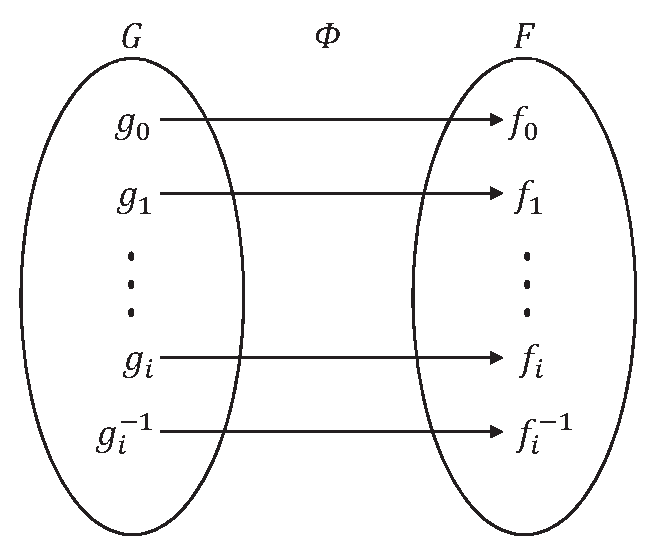
\includegraphics[width=0.4\linewidth]{fig/fig_D.1a.eps}
    }
    \quad
    \subfigure[同态关系]{
        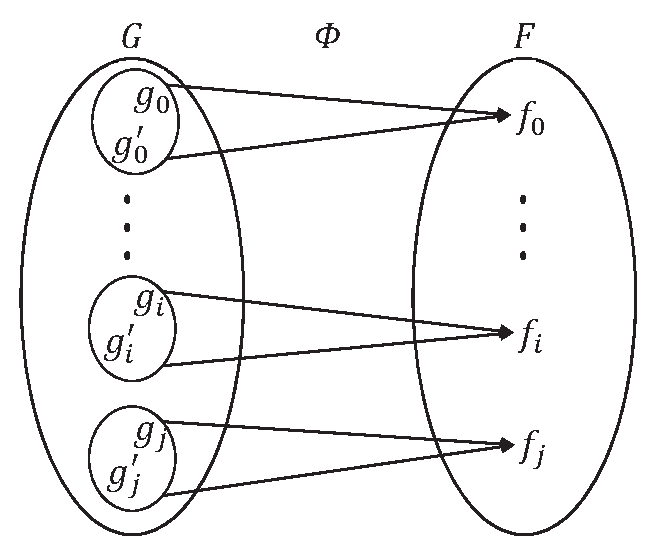
\includegraphics[width=0.4\linewidth]{fig/fig_D.1b.eps}
    }
    \caption{同构与同态}
    \label{fig:D.1}
\end{figure}
我们还可以很容易得到同态和同构映射的两个重要性质:
\begin{itemize}
    \item \textbf{幺元映射为幺元}:$\Phi(g_0)=f_0$
    \item \textbf{逆元映射为逆元}:$\Phi(g^{-1})=\Phi(g)^{-1}$
\end{itemize}
\begin{define}{同态核}
    $G$中所有与$F$中单位元素$f_0$所对应的元素的集合:
    \[\mathrm{Ker}\Phi\equiv\{h\in G|\Phi(h)=f_0\}\]
\end{define}
这个定义和线性代数里面线性映射的核(Kernel)\footnote{有的书也叫做零空间}的定义是类似的。
\begin{theorem}{同态核定理}
    设$G\cong F$,$H$是同态核,那么:
    \begin{itemize}
        \item $H\unlhd G$
        \item $G/H\cong F$
    \end{itemize}
    注意这个定理的表述默认$\Phi$是满的,否则要用$\mathrm{Im}\Phi$替换$F$
\end{theorem}
\begin{proof}
    第一点是比较容易证明的,首先不难$H$是子群,我们再稍微说明一下它是不变子群。我们要证明的实际上是$\forall h\in H,\forall g\in G\rightarrow ghg^{-1}\in H$,注意到
    $\Phi(ghg^{-1})=\Phi(g)\Phi(h)\Phi(g^{-1})=\Phi(g)\Phi(g^{-1})=f_0$,便直接证明$H\unlhd G$.

    第二点的证明我们实际上是需要去构建一个合适的同构映射,我们自然的可以想到这样的一个映射,将$G/H$中的元素$g_iH$映射到$\Phi(g_i)$上,你可以按照前面的图\ref{fig:D.1}理解为图b中的每一个小圈圈对应$G/H$中的一个
    陪集,构造的同构映射就是在同态映射的基础上将每个小圈圈对应$F$中的一个元素. 根据同态的性质,满性已然成立,下面要证明的是单性,也就是不同陪集对应不同元素.

    还是利用反证法来证明. 设$g_iH$和$g_jH$是两个不同的陪集,但是对应相同的$F$中元素$f$,那么$\forall h\in H, \Phi(g_i^{-1}g_jh)=f^{-1}ff_0=f_0\rightarrow g_i^{-1}g_jh\in H\rightarrow g_i^{-1}g_j\in H$,
    再根据重排定理,$g_i^{-1}g_jH=H\rightarrow g_iH=g_jH$,与假设矛盾.
    \qed
\end{proof}

看前面的图\ref{fig:D.1},这个定理实际上是在说与$F$中单位元素$f_0$对应的子群是$G$的一个不变子群,其它的小圈圈是他的陪集,所以每个小圈圈中的元素个数都相等,而且把这些小圈圈
单独看成一个个元素构成的商群和$F$同构。

\begin{define}{自然同态}
    如果$K\unlhd G$,那么映射$\pi:G\mapsto G/K$将$g$映射为陪集$gK$,建立了$G$和$G/K$之间的一个满同态\footnote[1]{也就是说$\mathrm{range}\pi=G/K$},而且同态核为
    $\mathrm{Ker}\pi=K$.我们称这个同态映射$\pi$为群$G$的自然同态.
\end{define}
这个实际上进一步告诉我们同态核和正规子群是一样的,也就是说一个正规子群可以看做某个群同态的同态核,反之同态核一定是某个正规子群。证明的话其实就是同态核定理逆推回去。
\begin{define}{自同构映射}
    自同构映射建立的是群和它自己的同构映射,$\nu :G\mapsto G$,最平凡的例子就是恒等映射。    
\end{define}
\begin{define}{自同构映射群}
    所有的自同构映射构成了一个群,乘法定义就是复合映射概念,我们记为$A(G)$.
\end{define}
\begin{define}{内自同构映射}
    还有一类同构映射比较特殊,$\forall u\in G$,我们可以依此构造一个自同构映射,我们定义映射为$\nu(g)=ugu^{-1}$,其实就是去找某个与$g$同类的元素。和上面类似的,自同构映射放在一起也构成了一个群,
    即自同构映射群,记为$I(G)$.
\end{define}
下面我们证明\textbf{内自同构映射群是自同构映射群的不变子群}。
\begin{proof}
    $I(G)\leq A(G)$这一点很容易证明,下面我们要证明$\forall \mu\in I(G),\nu\in A(G)\rightarrow\nu\mu\nu^{-1}\in I(G)$. 设$g_\alpha,g_\beta\in G, 
    \mu(g_\alpha)=u g_\alpha u^{-1},\nu(g_\alpha)=g_\beta$,那么$\nu\mu\nu^{-1}(g_\beta)=\nu\mu(g_\alpha)=\nu(ug_\alpha u^{-1})=\nu(u)g_\beta \nu(u)^{-1}$,
    根据$I(G)$的定义便得知$I(G)\unlhd A(G)$.
    \qed
\end{proof}
\subsection{群作用与变换群}
\begin{define}{左右作用与伴随作用}
    $\bigstar$左作用:$\forall g\in G$可以定义一个左作用$L_g:G\rightarrow G$,效果为$\forall g^\prime \in G,L_gg^\prime\equiv gg^\prime$.
    
    $\bigstar$右作用:$\forall g\in G$可以定义一个右作用$R_g:G\rightarrow G$,效果为$\forall g^\prime \in G,R_gg^\prime\equiv g^\prime g^{-1}$.

    $\bigstar$伴随作用:$\forall g\in G$可以定义一个伴随作用$\mathrm{Ad}_g:G\rightarrow G$,效果为$\forall g^\prime \in G,\mathrm{Ad}_gg^\prime\equiv gg^\prime g^{-1}$.
\end{define}
伴随作用就是前面说的内自同构映射的概念,也是三个作用里面最为重要的一个,而其它两个都不是同构映射。

\begin{define}{变换和变换群}
    设变换对象$X$是一个非空集合,则双射$f:X\rightarrow X$称为$X$上的一个变换或置换。定义这些置换的乘法为$f\circ g(x)=f(g(x))$,则所有的这些置换构成了一个群,
    称为$X$上的完全对称群$S_X$, 一般所说的变换群是$S_X$的子群。如果$X$有$n$个元素,则称其上的完全对称群为$X$上的$n$阶置换群$S_n$.如果我们变换的对象还构成一个群,
    它也有完全对称群$S_G$.
\end{define}

回到前面左右作用的定义,我们发现右作用不是直接右乘,而是右乘逆元。$\forall g\in G$,我们可以确定左右作用$L_g,R_g$,而这个确定给每个群元确定一个左(右)作用的过程其实就是一个$G\to S_G$的映射,当然这个映射不是满的,
但是却是个同态映射,很容易确定$L_{gg^\prime}=L_gL_{g^\prime}$,$R$同理。
\begin{theorem}{Cayley定理}
    群$G$同构于其完全变换群$S_G$的一个子群
\end{theorem}
\begin{proof}
    显然$G$中生成的左作用$L_g$构成的群$\{L_g|g\in G\}$就是这个子群而且与$G$同构.\qed
\end{proof}
\begin{define}{等价与轨道}
    设$G$为$X$上的变换群,若对$x,y\in X,\exists g\in G$,使得$g(x)=y$,那我们便称$x$与$y$等价,记为$x\sim y$. $X$中所有与$x$等价的元素的集合称为$x$的$G$轨道:
    $\mathcal{O}_x^G\equiv\{g(x)|g\in G\}$.
\end{define}
\begin{define}{不变子集}
    设$G$为$X$上的变换群,$Y\subseteq X$,满足$G$中的任意元素$g$作用在$Y$中元素上得到的结果还属于$Y$,那我们称$Y$为群$G$在$X$上的不变子集。
\end{define}
其实这个概念和线性代数里面的不变子空间概念是很像的。$\mathcal{O}_x^G$以及它们的并显然就是一些不变子集。
\begin{define}{迷向子群}
    设$G$为$X$上的变换群,$x\in X$,若$G^{x}\leq G$且保持$x$不变,即$G^{x}=\{h\in G|h(x)=x\}$,则称$G^{x}$是$G$对$x$的迷向子群。
\end{define}
\begin{define}{$\mathcal{O}_x^G$和$G^{x}$的左陪集一一对应}
    $G^{x}$的每个左陪集把$x$映为其$G$轨道上的点,且不同陪集映射到不同点。
\end{define}
由此我们便知$|\mathcal{O}_x^G|=|G|/|G^{x}|$.
\subsection{直积与半直积}
笛卡尔直积$\times$的概念就是两个集合中各取一个元素构成一个有序对来生成新的集合,我们进一步定义这个集合元素间的乘法是可以将其升级为群的。
\begin{define}{直积群}
    两个群中各取一个群元$g_{1\alpha},g_{2\beta}$构成一个有序对$g_{\alpha\beta}=(g_{1\alpha},g_{2\beta})$,且定义乘法,$g_{\alpha\beta}\times g_{\alpha^\prime\beta^\prime}
    =(g_{1\alpha}g_{1\alpha^\prime},g_{2\beta}g_{2\beta^\prime})$. 在这个乘法意义下这些有序对形成了一个新的群$G$,记为$G_1,G_2$的直积群$G_1\otimes G_2$.
\end{define}
\begin{define}{直积分解}
    若群$G$中的元素都可以唯一地拆写为$g_{\alpha\beta}=g_{1\alpha}g_{2\beta}$,其中$g_{1\alpha}\in G_1,g_{2\beta}\in G_2$,而且两个群之间的元素乘法满足交换律,即$\forall g_1\in G_1,g_2\in G_2\rightarrow g_1g_2=g_2g_1$,那
    自然的我们便将$G$中元素写成了有序对的形式,而且$G=G_1\otimes G_2$,$G_1,G_2$称为直积因子。
\end{define}
\begin{theorem}{直积因子的结构关系}
    群$G$的直积因子$G_1$和$G_2$满足:
    \begin{itemize}
        \item \textbf{只有一个公共元素幺元}:$G_1\cap G_2={e}$
        \item \textbf{都是正规子群}:$G_1\unlhd G, G_2\unlhd G$
    \end{itemize}
\end{theorem}
\begin{proof}
    第一点使用反证法证明,如果$G_1\cap G_2=a\neq e$,那么$G$中元素$a$可以写为$a=a\cdot e=e\cdot a$,都是前者属于$G_1$后者属于$G_2$,但显然拆分不唯一,不是直和分解定义。

    再看第二点,以$G_1$为例。$\forall g_1\in G,g=g_\alpha g_\beta\in G\rightarrow (g_\alpha g_\beta)g_1(g_\alpha g_\beta)^{-1}=g_{\alpha} g_1 g_{\alpha}^{-1}\in G_1$\qed
\end{proof}

\begin{define}{半直积}
    对于群$G_1$,如果$G_2\sim A(G_1)$,也就是说对于$G_2$中任意一个元素都能找到对应的一个$G_1$群的自同构映射$\nu_{g_{2\beta}}$.我们定义$G_1$和$G_2$之间元素构成的有序对集合$G=\{\left \langle g_{1\alpha},g_{2\beta}\right\rangle\}$
    之间的乘法满足
    \[\left\langle {{g_{1\alpha }},{g_{2\beta }}} \right\rangle  \times \left\langle {{g_{1\alpha '}},{g_{2\beta '}}} \right\rangle  = \left\langle {{g_{1\alpha }}{\nu _{{g_{2\beta }}}}({g_{1\alpha '}}),{g_{2\beta }}{g_{2\beta '}}} \right\rangle \]
    这样构造的新群称为$G_1,G_2$的半直积群,记为$G_1 \rtimes G_2$.
\end{define}
要证明这样定义乘法的正确性,注意$\nu_{g_{\beta}}(g_{\alpha}g_{\alpha^\prime})=\nu_{g_{\beta}}(g_{\alpha})\nu_{g_{\beta}}(g_{\alpha^\prime})$和$\nu_{g_\alpha g_\beta}=\nu_{g\alpha}\nu_{g_\beta}$即可。

从定义就可以看出来$G_1,G_2$的地位不是对称的,实际上这里$G_1\unlhd G$而$G_2$不再有这一性质。

\section{群表示论}